\documentclass[10pt,twocolumn,letterpaper]{article}

\usepackage{cvpr}
\usepackage{times}
\usepackage{epsfig}
\usepackage{graphicx}
\usepackage{amsmath}
\usepackage{amssymb}
\usepackage[utf8]{inputenc}
\usepackage{cite}
\usepackage{listings}
\usepackage[portuguese,ruled,lined]{algorithm2e}
\usepackage{spverbatim}

\renewcommand{\figurename}{Fig.}
\renewcommand{\refname}{Referências}
%\usepackage[breaklinks=true,bookmarks=false]{hyperref}

\cvprfinalcopy

\def\cvprPaperID{****}
%\def\httilde{\mbox{\tt\raisebox{-.5ex}{\symbol{126}}}}


\setcounter{page}{1}
\begin{document}

\title{\Huge Utilização do algoritmo PSO para ajuste dos pesos em redes RBF}

\author{Daniel Vilas-Boas\\
\footnotesize Departamento de Estatística e Informática\\
\footnotesize Universidade Federal Rural de Pernambuco\\
{\tt\small daanielvb@gmail.com}
\and
Leonardo Figueiroa\\
\footnotesize Departamento de Estatística e Informática\\
\footnotesize Universidade Federal Rural de Pernambuco\\
{\tt\small leonardofigueiroa@live.com}
\and
Rodrigo Cunha\\
\footnotesize Departamento de Estatística e Informática\\
\footnotesize Universidade Federal Rural de Pernambuco\\
{\tt\small r-cunha@outlook.com}
}

\maketitle
%\thispagestyle{empty}

\begin{abstract}
O uso de redes neurais de base radial ou RBFs vem sendo bastante utilizadas para classificação de padrões por apresentar diversas vantagens sobre outras redes (como a MLP), apresentando um treinamento mais eficiente e melhor grau de separabilidade. Este trabalho envolveu o desenvolvimento de uma RBF em conjunto com o algoritmo de otimização por enxame de partículas ou PSO. A rede neural foi desenvolvida de forma que seus pesos de saída fossem ajustados pelo PSO visando obter os melhores pesos na camada de saída e consequentemente menor taxa de erro e melhor classificação das características de entrada.\\
\begin{center}
\textbf{\textit{Palavras-chave --- RBF; PSO; redes neurais; classificação de padrões}}\\
\end{center}
\end{abstract}


\section{Introdução}
As redes denominadas \textit{funções de base radial}, convencionalmente conhecidas como \textit{RBF (radial basis function)}, são usadas em variados tipos de problemas tais como aproximação de funções e classificação de padrões. Ela pertence a arquitetura \textbf{feedforward} de camas múltiplas, cujo treinamento é efetivado de forma supervisionada. Sua estrutura é composta tipicamente por apenas uma camada intermediária, na qual as funções de ativação são do tipo \textit{gaussiana}. O fluxo de informações tem início na camada de entrada, passando então pela respectiva camada intermediária, e finalizando na camada neural de saída com neurônios com funções de ativação linear~\cite{livroAula}.\\ 

O \textit{PSO (Particle Swarm Optimization)} é um algoritmo de otimização por enxame de partículas. Tem uma abordagem \textbf{estocástica}, baseada em população que simula o processo comportamental de interação entre os indivíduos de um grupo. Sua teoria é baseada em comportamento de atividades de grupos de animais como pássaros e peixes, que realizam tarefas de otimização na execução de atividades como a busca por alimentos. O \textit{PSO} se inicia com um enxame de partículas com posições aleatórias. Cada partícula é dita ser uma possível solução para o problema investigado, sendo atribuído a cada indivíduo (partícula) um valor que está relacionado a adequação da partícula com a solução do problema (denominada \textbf{fitness}), e, também, uma variável velocidade que representa a direção do movimento da partícula. Com o passar do tempo, as partículas vão ajustando suas velocidades em relação a seu melhor \textbf{fitness}, encontrada pela própria partícula, e também pela melhor solução do grupo de partículas.\\ Elas continuam realizando este processo até que encontrem uma solução ótima. O valor \textbf{fitness} é definido pela natureza do problema de otimização e é computada por uma função objetivo que avalia um vetor solução. \\

Neste papel são discutidos a implementação da rede neural \textit{RBF} em conjunto com o algoritmo de otimização \textit{PSO}, os experimentos realizados após a implementação, e os resultados encontrados após os experimentos realizados.


%-------------------------------------------------------------------------
\subsection{Procedimentos}
Nesta seção serão discutidos os procedimentos realizados pela rede neural e pelo algoritmo de otimização. Os procedimentos são outros algoritmos conhecidos na literatura de \textbf{inteligência artificial} e \textbf{redes neurais artificiais} (como o \textit{kMeans} e a \textit{RBF}). Serão brevemente discutidos como funcionam e o seu papel na implementação do projeto. No \textbf{apêndice} pode ser encontrado o código-fonte do projeto para eventual consulta. O código-fonte está escrito em linguagem \textit{Java}.

\subsection{kMeans}

O primeiro procedimento realizado foi a \textbf{clusterização} das amostras por meio do algoritmo \textit{kMeans}. A partir de um valor $n$ que representa o número de centros na camada escondida da \textit{RBF} o algoritmo realiza a separação das amostras, calculando $n$ centros e suas respectivas variâncias.

\subsection{Cálculo das saídas intermediárias --- Y}

A partir dos centros das amostras e suas respectivas variâncias é utilizada a \textbf{função de base radial} para determinar o valor de saída da camada intermediária

$formula$

\subsection{Radial Basis Function --- RBF}
Pellentesque mauris sem, blandit tempor scelerisque nec, dictum sed lorem. Proin in libero a elit bibendum volutpat vitae a ligula. Aliquam sagittis ligula quis auctor sollicitudin. Sed eget blandit elit, ac sagittis dolor. Vestibulum in eros a nibh venenatis fermentum sit amet nec nibh. Suspendisse hendrerit cursus eros, eu ornare nisi placerat id. Phasellus venenatis eget velit eu consectetur. Sed elementum magna a venenatis cursus. Vivamus gravida viverra neque, et laoreet ipsum. Mauris pellentesque libero quis tincidunt ullamcorper. Donec egestas faucibus blandit. Morbi bibendum nibh eget dignissim congue. Sed maximus quis dolor quis congue. In hac habitasse platea dictumst.
\begin{figure}[h]
\begin{center}
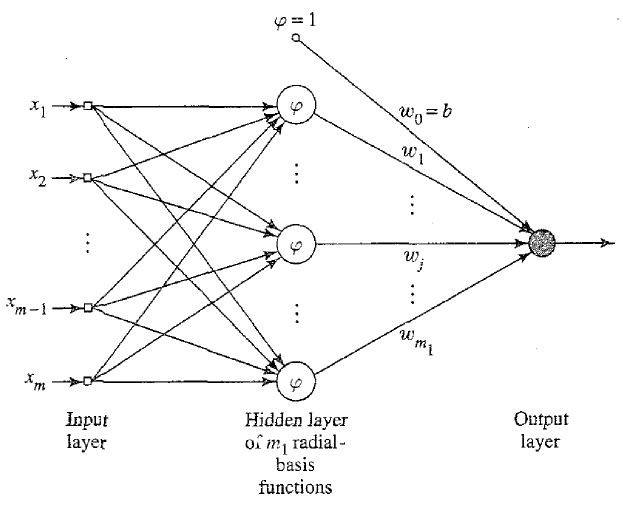
\includegraphics[scale=0.3]{foto1.jpg}
\caption{\textit{Estrutura teórica da RBF}}
\end{center}
\end{figure}
Pellentesque mauris sem, blandit tempor scelerisque nec, dictum sed lorem. Proin in libero a elit bibendum volutpat vitae a ligula. Aliquam sagittis ligula quis auctor sollicitudin. Sed eget blandit elit, ac sagittis dolor. Vestibulum in eros a nibh venenatis fermentum sit amet nec nibh. Suspendisse hendrerit cursus eros, eu ornare nisi placerat id. Phasellus venenatis eget velit eu consectetur. Sed elementum magna a venenatis cursus.

\subsection{Particle Swarm Optimisation --- PSO}
A otimização através de enxame de partículas é uma técnica \textbf{estocástica} baseada em processos comportamentais de grupos de animais criada pelo \textit{Dr. Eberhart} e  \textit{Dr. Kennedy} em 1995. O \textit{PSO} possui várias similaridades com as técnicas evolucionárias como os \textbf{Algoritmos Genéticos}, pois utiliza o conceito de vida artificial para interpretar comportamentos biológicos. Porém, apesar de possuir algumas similaridades como inicialização aleatória da população, a presença de um fator comparativo para avaliar a população (fitness) e atualização da população à medida que procuram pela solução ótima, diferenciam-se quanto a presença de operadores evolucionários como o \textbf{crossover} e a \textbf{mutação}. Isso resulta na evolução apenas da procura pela solução ótima e nao dos organismos em si.\\
O conceito é gerar uma coleção de partículas dentro de um espaço de função cujas dimensões são variáveis com o número de neurônios da camada escondida da \textit{RBF}. Cada partícula, então, segue o líder do enxame através da melhor partícula global em cada iteração, atualizando sua velocidade (e consequentemente sua posição) através das equações $(a)$ e $(b)$ que serão discutidas em breve. Nessa implementação \textbf{não} foram consideradas topologias de vizinhança para as partículas.~\cite{xiao}\\Abaixo, o algoritmo em pseudo-código do processo:

\begin{algorithm}[h!]
\Inicio{
\ParaCada {particula}{
inicialize a particula\;
}
\Repita{número de épocas ser atingido}{
\ParaCada{particula}{
calcule o valor do fitness\;
\Se {fitness for melhor $(\leq)$ que o fitness em pBest}{
guarde o valor como o novo pBest\;
}
}
Escolha a particula com melhor valor de fitness de todas as particulas como a gBest\;
\ParaCada {particula}{
calcule a velocidade de acordo com a equação (a)\;
atualize a posição de acordo com a equação (b)\;
}
}
}
\caption{Pseudo-código do PSO}
\end{algorithm}

Após as partículas serem inicializadas no espaço de função (intervalo de $-1 a 1$) é calculado o valor do \textbf{fitness} de cada partícula. O cálculo do valor é feito pela \textit{RBF} como o percentual de erro, discutido na seção acima.
Após o fitness ter sido calculado definimos o melhor global, que age como um fator de liderança para as demais partículas, e o melhor local da partícula (fator inércia). A partir deles, podemos calcular os vetores resultantes auxiliares e depois o vetor velocidade final que irá atualizar a posição da partícula no espaço. As equações de cálculo da velocidade e atualização da posição são dadas abaixo:

\begin{center}
\textit{(a)}\qquad$\vec{v} = \vec{v} + c_1 \times rand() \times (\vec{pBest} - \vec{pos}) + c_2 \times rand() \times (\vec{gBest - \vec{pos}})$ 
\end{center}

Onde $\vec{v}$ é o vetor velocidade, $c_1$ e $c_2$ são fatores de aprendizado ($c_1 = c_2 = 2$), $rand()$ é uma função que irá gerar um valor aleatório no intervalo 0---1, $\vec{pBest}$ e $\vec{gBest}$ são os vetores de posição do melhor local e global respectivamente, e $\vec{pos}$ é o vetor posição atual da partícula. 

\begin{center}
\textit{(b)}\qquad$\vec{pos} = \vec{pos_{ant}} + \vec{v}$ 
\end{center}
Onde $\vec{pos}$ é o vetor posição atual da partícula a ser atualizado, $\vec{pos_{ant}}$ é o vetor posição anterior a atualização, e $\vec{v}$ é o vetor velocidade calculado através da equação $(a)$.
%-------------------------------------------------------------------------

\section{Experimentos}

\subsection{Variando o número de neurônios, épocas e partículas}
Pellentesque mauris sem, blandit tempor scelerisque nec, dictum sed lorem. Proin in libero a elit bibendum volutpat vitae a ligula. Aliquam sagittis ligula quis auctor sollicitudin. Sed eget blandit elit, ac sagittis dolor. Vestibulum in eros a nibh venenatis fermentum sit amet nec nibh. Suspendisse hendrerit cursus eros, eu ornare nisi placerat id. Phasellus venenatis eget velit eu consectetur. Sed elementum magna a venenatis cursus. Vivamus gravida viverra neque, et laoreet ipsum. Mauris pellentesque libero quis tincidunt ullamcorper. Donec egestas faucibus blandit. Morbi bibendum nibh eget dignissim congue. Sed maximus quis dolor quis congue. In hac habitasse platea dictumst.

Nullam pulvinar nunc nec interdum sodales. Cras elit erat, gravida id tortor eu, molestie volutpat felis. Duis quis ipsum sapien. Etiam nec porttitor est. Vestibulum neque leo, sagittis id interdum vitae, congue a mi. Vestibulum interdum ipsum id viverra egestas. Suspendisse iaculis turpis nibh, a viverra dolor tempor eget. Donec volutpat, sapien a auctor venenatis, justo enim gravida nisi, vitae laoreet ipsum ligula sit amet mauris. Proin rhoncus auctor lectus, in dignissim elit.

\subsection{Observações}
Nullam pulvinar nunc nec interdum sodales. Cras elit erat, gravida id tortor eu, molestie volutpat felis. Duis quis ipsum sapien. Etiam nec porttitor est. Vestibulum neque leo, sagittis id interdum vitae, congue a mi. Vestibulum interdum ipsum id viverra egestas.

\section{Conclusão}

Nullam pulvinar nunc nec interdum sodales. Cras elit erat, gravida id tortor eu, molestie volutpat felis. Duis quis ipsum sapien. Etiam nec porttitor est. Vestibulum neque leo, sagittis id interdum vitae, congue a mi. Vestibulum interdum ipsum id viverra egestas. Suspendisse iaculis turpis nibh, a viverra dolor tempor eget. Donec volutpat, sapien a auctor venenatis, justo enim gravida nisi, vitae laoreet ipsum ligula sit amet mauris. Proin rhoncus auctor lectus, in dignissim elit.

{\small
\bibliographystyle{ieee}
\bibliography{rna}
}

\newpage
\onecolumn
   
\section*{Apêndice}
Aqui encontram-se os códigos escritos durante a implementação do projeto.
\section*{Pacote kmeans --- AuxiliaryFunctions.java}

\begin{spverbatim}
package kmeans;

public class AuxiliaryFunctions {
	
	/*
	 * Euclidean distance in 4 dimensions between Ponto
	 */
	public static double calculateEuclideanDistance4Dimensions(Ponto v, Ponto w){
		double result = Math.sqrt(Math.pow((w.getX() - v.getX()),2) + Math.pow((w.getY() - v.getY()),2) +
						Math.pow((w.getZ() - v.getZ()),2) + Math.pow((w.getW() - v.getW()),2) );
		return result;
	}
	
	/*
	 * Eucliadean distance in 4 dimensions between Ponto and Cluster
	 */
	public static double calculateEuclideanDistance4Dimensions(Ponto v, Cluster c){
		double result = Math.sqrt(Math.pow((c.getCenter().getX() - v.getX()),2) + Math.pow((c.getCenter().getY() - v.getY()),2) +
						Math.pow((c.getCenter().getZ() - v.getZ()),2) + Math.pow((c.getCenter().getW() - v.getW()),2) );
		return result;
	}
	
	/*
	 * Calculates RBF weights between input and intermediate layers
	 */
	public static double calculateRBFWeights(Ponto centro,Ponto p,double varianca ){
		return Math.exp(-Math.pow(calculateEuclideanDistance4Dimensions(centro,p),2)/2* (Math.pow(varianca,2)));
	}
}
\end{spverbatim}

\section*{Pacote kmeans --- Cluster.java}

\begin{spverbatim}
package kmeans;

import java.util.ArrayList;

public class Cluster {
	private Ponto center;
	private ArrayList<Ponto> contains;
	private Double variance;
	
	//Constructor
	
	

	public Cluster(ArrayList <Ponto> ar,int size){
		int index = (int)(Math.random()*size);
		Ponto pt = ar.get(index);
		
		this.center = pt;
		this.contains = new ArrayList<Ponto>();
		
	}
	
	//Adds Ponto to itself
	
	public void addPonto(Ponto p){
		this.contains.add(p);
	}
	
	//Recalculate new center based on its points mean 
	
	public void CalculateNewCenter(){
		int size = this.contains.size();
		if(size == 0){
			//System.out.println("Empty Cluster");
		}
		else{
		double sumX = 0;
		double sumY = 0;
		double sumZ = 0;
		double sumW = 0;
		for (int i = 0; i < size ; i++){
			sumX += this.contains.get(i).getX();
			sumY += this.contains.get(i).getY();
			sumZ += this.contains.get(i).getZ();
			sumW += this.contains.get(i).getW();
		}
		this.center.setX(sumX/size);
		this.center.setY(sumY/size);
		this.center.setZ(sumZ/size);
		this.center.setW(sumW/size);
	}
	}
	
	//Verify if the Cluster has changed position
	
	public boolean hasChangedPosition(){
		double oldx = this.center.getX();
		double oldy = this.center.getY();
		double oldz = this.center.getZ();
		double oldw = this.center.getW();
		this.CalculateNewCenter();
		if(this.getCenter().getX() == oldx && this.getCenter().getY() == oldy &&
			this.getCenter().getZ() == oldz && this.getCenter().getW() == oldw){
			return false;
		}
		return true;
	}
	
	public void calculateVariance(){
		if(this.getContains().size() == 0){
			this.variance = 0.0;
		}
		else{
			Double sum = 0.0 ;
			for (int i = 0; i < this.getContains().size(); i++) {
				sum += AuxiliaryFunctions.calculateEuclideanDistance4Dimensions(this.getCenter(), this.getContains().get(i));
			}
			this.variance = sum/this.getContains().size();
		}
	}
	// Getters & setters
	
	public Ponto getCenter() {
		return center;
	}
	public void setCenter(Ponto center) {
		this.center = center;
	}
	public ArrayList<Ponto> getContains() {
		return contains;
	}
	public void setContains(ArrayList<Ponto> contains) {
		this.contains = contains;
	}
	
	public Double getVariance() {
		return variance;
	}

	public void setVariance(Double variance) {
		this.variance = variance;
	}
	
}
\end{spverbatim}

\section*{Pacote kmeans --- Kmeans.java}

\begin{spverbatim}
package kmeans;

import java.io.FileNotFoundException;
import java.util.ArrayList;



public class Kmeans {
	private ArrayList<Ponto> database;
	private ArrayList<Cluster> clusters;
	
	//Constructor
	
	public Kmeans(){
		this.database = new ArrayList<Ponto>();
		this.clusters = new ArrayList<Cluster>();
	}
		
	//Add Ponto to database
	
	public void addPonto(Ponto p){
		this.database.add(p);
	}
	

	//Generate clusters
	
	public void generateKClusters(int k){
		for (int i = 0; i < k; i++){
			this.clusters.add(new Cluster(this.database,this.database.size()));
		}
	}

	
	
	//Calculate Distance from every single Ponto to every Cluster
	public void calculateRelativeDistances(){
		for(int i = 0;i < this.database.size(); i++){
			for(int j=0; j < this.clusters.size(); j++){
				//this.database.get(i).addRelativeDistances(calculateDist(this.database.get(i),
				this.clusters.get(j)));
this.database.get(i).addRelativeDistances(AuxiliaryFunctions.
				calculateEuclideanDistance4Dimensions(this.database.get(i), this.clusters.get(j)));
			}
		}
	}
	
	
	
	//Insert Ponto into the closest Cluster
	
	public void insertIntoClusters(){
		for(int i = 0; i < this.database.size(); i++){
			int index = this.database.get(i).getClosestElementIndex();
			this.clusters.get(index).addPonto(this.database.get(i));
		}
	}
	
	
	// Recalculate Clusters centers after Ponto addition
	
	public boolean recalculateClusters(){
		for(int i = 0; i < this.clusters.size(); i++){
			boolean flag = this.clusters.get(i).hasChangedPosition();
			if (flag){
				return true;
			}
	}
		return false;
	}
	
	// Clears Clusters' contains
	
	public void clearClusters(){
		for(int i = 0; i < this.clusters.size(); i++){
			this.clusters.get(i).getContains().clear();
			}
	}
	
	// Clear Pontos
	
		public void clearPontos(){
			for(int i = 0; i < this.database.size(); i++){
				this.database.get(i).getDistances().clear();
				}
		}
		
	/*
	 * When kmeans object is created the whole algorithm starts
	 */
	public void kmeans(int k,ArrayList<Ponto> db) throws FileNotFoundException{
		
		this.setDatabase(db);
		this.generateKClusters(k);
		boolean flag = true;
		
		//kmeans computing
		while (flag)
		{
			this.calculateRelativeDistances();
			this.insertIntoClusters();
			flag = this.recalculateClusters();
			if (flag)
			{
				this.clearClusters();
				this.clearPontos();
			}
		}
		
		//Variance
		for (int i = 0; i < this.getClusters().size(); i++) {
			this.getClusters().get(i).calculateVariance();
			
		}
	}
	
	/*
	 * Prints clusters centers and variance
	 */
	public String printAllClustersCenter()
	{
		String str = "";
		for (int i = 0; i < this.getClusters().size(); i++)
			str = str + this.getClusters().get(i).getCenter().printCoordinates() + "\n";
		return str;
	}
	
	public String printAllClustersVariance()
	{
		String str = "";
		for (int i = 0; i < this.getClusters().size(); i++)
			str = str + this.getClusters().get(i).getVariance() + "\n";
		return str;
	}
	
	// Getters & setters

	public ArrayList<Ponto> getDatabase() {
		return database;
	}


	public void setDatabase(ArrayList<Ponto> database) {
		this.database = database;
	}


	public ArrayList<Cluster> getClusters() {
		return clusters;
	}


	public void setClusters(ArrayList<Cluster> clusters) {
		this.clusters = clusters;
	}

}
\end{spverbatim}

\section*{Pacote kmeans --- Ponto.java}

\begin{spverbatim}
package kmeans;

import java.util.ArrayList;


public class Ponto {
		private double x;
		private double y;
		private double z;
		private double w;
		private ArrayList<Double> distances;
		
		// Constructor 
		
		public Ponto(double x,double y,double z,double w){
			this.x = x;
			this.y = y;
			this.z = z;
			this.w = w;
			this.distances = new ArrayList<Double>();
		}
		
		public Ponto(ArrayList<Double> entrada){
			this.x = entrada.get(0);
			this.y = entrada.get(1);
			this.z = entrada.get(2);
			this.w = entrada.get(3);
			this.distances = new ArrayList<Double>();
		}
		
		// Adds a new distance to the relativeDistances Array
		
		public void addRelativeDistances(double dist){
			this.distances.add(new Double(dist));
		}
		
		// Auxiliary functions to get smallest distance element and index 
		
		public double getClosest(){
			double min = this.distances.get(0);
			for(int i = 0; i < this.distances.size(); i++){
				if(this.distances.get(i) < min){
					min = distances.get(i);
				}
			}
			return min;
		}
		
		public int getClosestElementIndex(){
			double min = this.distances.get(0);
			int index = 0;
			for(int i = 0; i < this.distances.size(); i++){
				if(this.distances.get(i) < min){
					min = distances.get(i);
					index = distances.indexOf(min);
				}
			}
			return index;
		}
		
		public String printCoordinates(){
			return " X:" + this.x + " Y:" + this.y + " Z: " + this.z + " W:" + this.w;
		}
		// Getters & setters
		public double getX() {
			return x;
		}
		public void setX(double x) {
			this.x = x;
		}
		public double getY() {
			return y;
		}
		public void setY(double y) {
			this.y = y;
		}
		
		public double getZ() {
			return z;
		}

		public void setZ(double z) {
			this.z = z;
		}

		public double getW() {
			return w;
		}

		public void setW(double w) {
			this.w = w;
		}

		public ArrayList<Double> getDistances() {
			return distances;
		}
		public void setDistances(ArrayList<Double> distances) {
			this.distances = distances;
		}

}
\end{spverbatim}

\section*{Pacote pso --- Particula.java}

\begin{spverbatim}
package pso;

import java.util.Arrays;
import java.util.Random;

public class Particula {

	private double fitness; // solucao encontrada (taxa de erro medio da RBF)
	private Particula pBest; // melhor solucao ja encontrada pela particula (posicao e fitness guardados)
	private double[] posicao;
	private double[] velocidade;
	

	public Particula(int numNeuronios) { //construtor
		
		this.posicao = new double[numNeuronios];
		this.velocidade = new double[numNeuronios];
		this.fitness = 3; // ja que a taxa de erro pode estar entre 0 e 2. necessario inicializar assim por causa da primeira comparacao do metodo define_pBest.
		for (int i = 0; i < this.posicao.length; i++) { 
			Random numRandom = new Random(); // preenche aleatoriamente o vetor de coordenadas d-dimensional da particula
			this.posicao[i] = (numRandom.nextDouble() * 2) - 1; // intervalo [-1, 1]
			this.velocidade[i] = 0;
		}
	}
	
	public void calculaVelocidade(){
		// da equacao v[] = v[] + c1 * rand() * (pbest[] - present[]) + c2 * rand() * (gbest[] - present[])
		Random random = new Random();
		double c1 = 2 * random.nextDouble();
		double c2 = 2 * random.nextDouble();
		
		double[] d_pBest = new double [this.posicao.length]; // vetor pBest
		double[] d_gBest = new double [this.posicao.length]; // vetor gBest
		
		//decidi fazer varios lacos for para melhorar a legibilidade da equacao
		
		for (int i = 0; i < d_pBest.length; i++) { // subtrai os vetores pBest e posicao utilizando o metodo do triangulo e multiplica pelo fator de aprendizado c1
			d_pBest[i] = this.posicao[i] * (-1);
			d_pBest[i] = d_pBest[i] + pBest.getPosicao()[i];
			d_pBest[i] = d_pBest[i] + c1;
		}
		
		for (int i = 0; i < d_gBest.length; i++) { // subtrai os vetores gBest e posicao utilizando o metodo do triangulo e multiplica pelo fator de aprendizado c2
			d_gBest[i] = posicao[i] * (-1);
			d_gBest[i] += Pso.gBest.posicao[i];
			d_gBest[i] += c2;
		}
		
		for (int i = 0; i < d_pBest.length; i++) { // soma os vetores d_pBest e d_gBest e salva em d_pBest como um vetor resultante
			d_pBest[i] += d_pBest[i] + d_gBest[i];
		}
		
		for (int i = 0; i < this.velocidade.length; i++) { // finalmente, soma os vetores d_pBest velocidade
			this.velocidade[i] += d_pBest[i];
		}
		
		/*System.out.println("vetor d_pBest" + Arrays.toString(d_pBest));
		System.out.println("vetor d_gBest" + Arrays.toString(d_gBest));
		System.out.println("vetor velocidade" + Arrays.toString(velocidade));
		System.out.println("vetor pBest posicao" + Arrays.toString(pBest.posicao));
		System.out.println("vetor gBest posicao" + Arrays.toString(Pso.gBest.posicao));*/
	}
	
	public void deslocarParticula(){
		for (int i = 0; i < this.posicao.length; i++) {
			this.posicao[i] = this.pBest.posicao[i] + this.velocidade[i];
		}
	}
	
	public double getFitness() {
		return fitness;
	}

	public void setFitness(double fitness) {
		this.fitness = fitness;
	}

	public Particula getpBest() {
		return pBest;
	}

	public void setpBest(Particula pBest) {
		this.pBest = pBest;
	}

	public double[] getPosicao() {
		return posicao;
	}

	public void setPosicao(double[] posicao) {
		this.posicao = posicao;
	}

	public double[] getVelocidade() {
		return velocidade;
	}

	public void setVelocidade(double[] velocidade) {
		this.velocidade = velocidade;
	}
}
\end{spverbatim}

\section*{Pacote pso --- Pso.java}

\begin{spverbatim}
package pso;

import java.util.ArrayList;
import java.util.Arrays;

/* PSO: tecnica de otimizacao do tipo estocastica (aleatoria) inspirada no comportamento social
 * de . Possui muitas similaridades com tecnicas de evolucao computacional, como os Algoritmos
 * Geneticos.
 * 
 * http://www.swarmintelligence.org/
 * 
 * O PSO possui uma populacao (enxame) de solucoes candidatas (as particulas). As particulas
 * movem-se no espaco de busca de acordo com algumas formulas simples. Os movimentos das par-
 * ticulas sao guiados pela sua melhor posicao conhecida no espaco de busca, assim como a melhor
 * posicao conhecida do enxame. O pocesso e repetido e, e esperado, mas nao garantido, que uma
 * solucao satisfatoria sera, eventualmente, descoberta.
 * 
 * https://en.wikipedia.org/wiki/Particle_swarm_optimization
 * 
 * ---------------------------------------------------------------------------------------------
 * Pseudo-codigo:
 * 
 * For each particle 
 * 	Initialize particle
 * END
 *	
 * Do
 *	For each particle 
 *		Calculate fitness value
 *	    If the fitness value is better than the best fitness value (pBest) in history
 *	        set current value as the new pBest
 *	End
 *	
 *	Choose the particle with the best fitness value of all the particles as the gBest
 *	For each particle 
 *	   Calculate particle velocity according equation (a)
 *	   Update particle position according equation (b)
 *   End 
 * While maximum iterations or minimum error criteria is not attained
 * 
 * http://www.swarmintelligence.org/tutorials.php
 * 
 * ---------------------------------------------------------------------------------------------
 * Equacoes:
 * - Velocidade (a):
 * 		v[] = v[] + c1 * rand() * (pbest[] - present[]) + c2 * rand() * (gbest[] - present[])
 * - Posicao (b):
 *  	present[] = persent[] + v[]
 *  
 *  v[] is the particle velocity, persent[] is the current particle (solution).
 *  pbest[] *  and gbest[] are defined as stated before.
 *  rand () is a random number between (0,1).
 *  c1, c2 are learning factors. usually c1 = c2 = 2.
 *   
 *  http://www.swarmintelligence.org/tutorials.php
 */
public class Pso {

	public static Particula gBest; // Particula com melhor fitness do enxame (posicao e fitness guardados)
	private ArrayList<Particula> enxame;
	private final double v_min = -2;
	private final double v_max = 2;
	
	public Pso(int numNeuronios, int numEpocas, int numParticulas) {
		criaEnxame(numParticulas, numNeuronios);
		gBest = new Particula(numNeuronios);
		gBest.setFitness(enxame.get(0).getFitness());
		gBest.setPosicao(enxame.get(0).getPosicao().clone());
		System.out.println(Arrays.toString(gBest.getPosicao()));
		for (int i = 0; i < enxame.size(); i++) {
			enxame.get(i).setpBest(enxame.get(i));
		}
		
		for (int i = 0; i < numEpocas; i++) {
			for (int j = 0; j < this.enxame.size(); j++) {
				this.enxame.get(j).setFitness(rbf.RBF.calculateErrorPercentage(this.enxame.get(j), numNeuronios)); // calcula o fitness da particula
				define_pBest(this.enxame.get(j));
			}
			define_gBest();
			for (int j = 0; j < this.enxame.size(); j++) {
				this.enxame.get(j).calculaVelocidade();
				for (int k = 0; k < this.enxame.get(j).getVelocidade().length; k++) {
					if (this.enxame.get(j).getVelocidade()[k] < v_min){
						this.enxame.get(j).getVelocidade()[k] = v_min;
						//System.out.println("entrou if 1 " + enxame.get(j).getVelocidade()[k]);
					}else if (this.enxame.get(j).getVelocidade()[k] > v_max){
						this.enxame.get(j).getVelocidade()[k] = v_max;
						//System.out.println("entrou if 2 " + enxame.get(j).getVelocidade()[k]);
					}
				}
				this.enxame.get(j).deslocarParticula();
			}
		}
	}

	private void criaEnxame(int numParticulas, int numNeuronios) {
		this.enxame = new ArrayList<Particula>();
		// cria um enxame com n particulas (definido pelo usuario; geralmente
		// entre 20 e 50) que sao d-dimensionais (definido pelo numero de
		// neurinios da camada escondida da rbf).
		Particula p;
		for (int i = 0; i < numParticulas; i++) {
			p = new Particula(numNeuronios); // ja com a posicao aleatoria
			this.enxame.add(p);
		}
	}

	public void define_gBest() { // define quem eh a particula gBest e guarda uma copia
		for (int i = 0; i < this.enxame.size(); i++) {
			if (this.enxame.get(i).getFitness() < gBest.getFitness()) {
				gBest.setPosicao(this.enxame.get(i).getPosicao().clone());
				gBest.setFitness(this.enxame.get(i).getFitness());
				System.out.println("Trocou gBest");
				System.out.println(gBest.getFitness());
				System.out.println(Arrays.toString(gBest.getPosicao()));
				
			}
		}
	}
	
	public void define_pBest(Particula p){
		if (p.getFitness() < p.getpBest().getFitness()) {
			p.getpBest().setPosicao(p.getPosicao().clone());
			p.getpBest().setFitness(p.getFitness());
			System.out.println("Trocou pBest");
		}
	}

	public ArrayList<Particula> getEnxame() {
		return enxame;
	}

	public void setEnxame(ArrayList<Particula> enxame) {
		this.enxame = enxame;
	}
}
\end{spverbatim}

\section*{Pacote rbf --- LeitorEntrada.java}

\begin{spverbatim}
package rbf;

import java.io.BufferedReader;
import java.io.FileReader;
import java.io.IOException;
import java.util.ArrayList;

import kmeans.Ponto;

public class LeitorEntradaRBF {
	private ArrayList<ArrayList <Double>> baseEntrada;
	private ArrayList<Ponto> conjuntoCaracteristicas;
	private int tamanho;
	
	public LeitorEntradaRBF(){
		this.baseEntrada = new ArrayList<ArrayList <Double>>();
		this.conjuntoCaracteristicas = new ArrayList<Ponto>();
	}
	
	/*
	 * Converts database to ArrayList<Double>
	 */
	public void lerEntrada(){
		BufferedReader br = null;
		try {
			String sCurrentLine;
			br = new BufferedReader(new FileReader("TreinaIris.txt"));
			while ((sCurrentLine = br.readLine()) != null) {
				// parts representa uma linha da base [d,d,d,d,c]
				String[] parts = sCurrentLine.split("\t");
				ArrayList<Double> amostra = new ArrayList<Double>();
				for (int i = 0; i < parts.length; i++) {							
					amostra.add(Double.valueOf(parts[i]));	
					
				}
				this.baseEntrada.add(amostra);	
			}
			this.setTamanho(this.baseEntrada.size());

		} catch (IOException e) {
			e.printStackTrace();
		} finally {
			try {
				if (br != null)br.close();
			} catch (IOException ex) {
				ex.printStackTrace();
	}

}
	}
	
	/*
	 * Converts current database read to ArrayList<Ponto>
	 */
	public void converterBaseParaPonto(){
		for (int i = 0; i < this.getBaseEntrada().size(); i++) {
			ArrayList<Double> temp = new ArrayList<Double>();
			for (int j = 0; j <= 3 ; j++) {
				temp.add(this.getBaseEntrada().get(i).get(j));
			}
			Ponto p = new Ponto(temp);
			this.getConjuntoCaracteristicas().add(p);
		}
		
	}
	
	public ArrayList<Ponto> getConjuntoCaracteristicas() {
		return conjuntoCaracteristicas;
	}

	public void setConjuntoCaracteristicas(ArrayList<Ponto> conjuntoCaracteristicas) {
		this.conjuntoCaracteristicas = conjuntoCaracteristicas;
	}

	public ArrayList<ArrayList<Double>> getBaseEntrada() {
		return baseEntrada;
	}


	public void setBaseEntrada(ArrayList<ArrayList<Double>> baseEntrada) {
		this.baseEntrada = baseEntrada;
	}


	public int getTamanho() {
		return tamanho;
	}

	public void setTamanho(int tamanho) {
		this.tamanho = tamanho;
	}
}
\end{spverbatim}

\section*{Pacote rbf --- RBF.java}

\begin{spverbatim}
package rbf;

import java.util.ArrayList;
import java.util.List;

import kmeans.AuxiliaryFunctions;
import kmeans.Cluster;
import kmeans.Kmeans;
import kmeans.Ponto;
import pso.Particula;

public class RBF {
	private static List<Cluster> rbfs;
	private static LeitorEntradaRBF leitorEntrada;
	static int contador = 0;

	public RBF(Kmeans k, LeitorEntradaRBF leitor) {
		this.rbfs = k.getClusters();
		this.leitorEntrada = leitor;
		
	}

	/*
	 * Varre a base de entrada e o numero de neuronios para calcular os pesos
	 * intermediarios e posteriormente o % de erro
	 */
	public static double calculateErrorPercentage(Particula p, int numNeuronios) {
		double erro = 0;
		for (int j = 0; j < getLeitorEntrada().getConjuntoCaracteristicas().size(); j++) {
			// Array com valores temporarios de Y
			ArrayList<Double> Y = new ArrayList<Double>();
			for (int i = 0; i < numNeuronios; i++) {
				Y.add(AuxiliaryFunctions.calculateRBFWeights(getRbfs().get(i).getCenter(), // c
						getLeitorEntrada().getConjuntoCaracteristicas().get(j),
						getRbfs().get(i).getVariance()));
			}
			// Somatorio das multiplicacoes de Y x W
			double somatorio = 0;
			for (int z = 0; z < Y.size(); z++) {
				somatorio += p.getPosicao()[z] * Y.get(z);
			}
			erro += Math.abs(getLeitorEntrada().getBaseEntrada().get(j).get(4) - somatorio);
			// System.out.println("erro antes do return: " + erro);
		}
		//contador++;
		
		erro = erro / getLeitorEntrada().getBaseEntrada().size();
		//System.out.println("erro depois do return: " + erro);
		//System.out.println(contador);
		//return erro / getLeitorEntrada().getBaseEntrada().size();
		return erro;
	}

	public static List<Cluster> getRbfs() {
		return rbfs;
	}

	public void setRbfs(List<Cluster> rbfs) {
		this.rbfs = rbfs;
	}

	public static LeitorEntradaRBF getLeitorEntrada() {
		return leitorEntrada;
	}

	public void setLeitorEntrada(LeitorEntradaRBF leitorEntrada) {
		this.leitorEntrada = leitorEntrada;
	}

}
\end{spverbatim}

\section*{Pacote testes --- TestClass.java}

\begin{spverbatim}
package testes;

import java.io.FileNotFoundException;

import kmeans.Kmeans;
import pso.Particula;
import rbf.LeitorEntradaRBF;
import rbf.RBF;

public class TestClass {

	public static void main(String[] args) throws FileNotFoundException {
		LeitorEntradaRBF le = new LeitorEntradaRBF();
		le.lerEntrada();
		le.converterBaseParaPonto();
		Kmeans k = new Kmeans();
		k.kmeans(4, le.getConjuntoCaracteristicas());
		RBF rbf = new RBF(k,le);
		for (int i = 0; i < 15; i++) {
			Particula p = new Particula(4);
			System.out.println(rbf.calculateErrorPercentage(p, 4));
		}
		
		
//		
		
		
		System.out.println(rbf.getLeitorEntrada().getConjuntoCaracteristicas().size());

	}

}
\end{spverbatim}

\section*{Pacote testes --- Teste.java}

\begin{spverbatim}
package testes;

import java.io.FileNotFoundException;
import java.util.Arrays;

import kmeans.Kmeans;
import pso.Particula;
import pso.Pso;
import rbf.LeitorEntradaRBF;
import rbf.RBF;

public class Teste {

		public static void main(String[] args) throws FileNotFoundException {
			LeitorEntradaRBF le = new LeitorEntradaRBF();
			le.lerEntrada();
			le.converterBaseParaPonto();
			Kmeans k = new Kmeans();
			k.kmeans(4, le.getConjuntoCaracteristicas()); // primeiro argumento deve ser igual ao numNeuronios
			RBF rbf = new RBF(k, le);
			
			/*for (int i = 0; i < 15; i++) {
				Particula p = new Particula(4);
				//System.out.println(rbf.calculateErrorPercentage(p, 4));
			}*/
			
			//System.out.println(Pso.FuncaoGeral(4, 10, 20));
			/*System.out.println(Arrays.toString(Pso.FuncaoGeral(1, 2, 1).posicao));
			System.out.println(Pso.gBest.fitness);
			System.out.println(Arrays.toString(Pso.gBest.posicao));
			System.out.println(Arrays.toString(Pso.gBest.velocidade));
			System.out.println(Pso.gBest);*/
			
			Pso pso = new Pso(4, 100, 25);
			
			//System.out.println(pso.gBest.getFitness());
			//System.out.println(Arrays.toString(pso.gBest.getPosicao()));

		}

	}
\end{spverbatim}
\end{document}
